% Generated by scireport <version> (template generic@1, layout default@1) from a bundle with manifest sha256 7112702977a0. Do not edit.
\documentclass[10pt]{article}
\usepackage[a4]{scireport-default}
\hypersetup{pdftitle={Full-kinds report},%
pdfauthor={N. Cardoso},%
pdfkeywords={compat, spec-1.0},%
pdflang={en},%
  pdfcreator={scireport <version>}}
\scsetrunning{compat corpus}{N. Cardoso}{scireport compat corpus, spec 1.0}
\begin{document}
\sccover{compat corpus}{Full-kinds report}{Every v1.0 kind}{N. Cardoso\par }{Date & 2026-10-09\\Version & 1.0.0\\Keywords & compat, spec-1.0\\}

\par{\fontsize{14}{17}\selectfont\bfseries Abstract}\par\vspace{4pt}
A report that exercises \textbf{every} kind.
\clearpage
\scanchor{sc-toc}{Contents}{}%
{\fontsize{20}{24}\selectfont\bfseries\color{sc-navy}Contents\par}%
\vspace{2pt}\scrule{sc-gray-200}{1pt}\vspace{4pt}
\sctocrow{0}{01}{Values}{a1}

Short \textbf{markdown} text.

\scchapter{01}{Values}{a1}{Values}{0}

\noindent{\bfseries\color{sc-ink-soft}Number:} 1.23 \ensuremath{\pm} 0.01~arcsec\par

{\fontsize{8}{11}\selectfont\renewcommand{\arraystretch}{1.45}
\setlength{\sctablew}{\scfullwidth}\begin{longtable}{>{\raggedleft\arraybackslash\ttfamily}p{\dimexpr 0.33333\sctablew-2\tabcolsep\relax}>{\raggedleft\arraybackslash\ttfamily}p{\dimexpr 0.33333\sctablew-2\tabcolsep\relax}>{\raggedright\arraybackslash}p{\dimexpr 0.33333\sctablew-2\tabcolsep\relax}}
\rowcolor{sc-gray-50}{\bfseries\color{sc-ink-soft}ID} & {\bfseries\color{sc-ink-soft}Redshift} & {\bfseries\color{sc-ink-soft}label} \\
\scheadrule
\endfirsthead
\rowcolor{sc-gray-50}{\bfseries\color{sc-ink-soft}ID} & {\bfseries\color{sc-ink-soft}Redshift} & {\bfseries\color{sc-ink-soft}label} \\
\scheadrule
\endhead
1 & 0.100 & a \\
\scrowrule
2 & -- & b \\
\scrowrule
3 & 0.300 & c \\
\scrowrule
\end{longtable}}
\begin{adjustwidth}{0pt}{-\scoverhang}\vspace{-8pt}\setcounter{table}{0}\captionof{table}{A Parquet table}\end{adjustwidth}

\begin{adjustwidth}{0pt}{-\scoverhang}
\begin{samepage}
\vspace{16pt}\centering
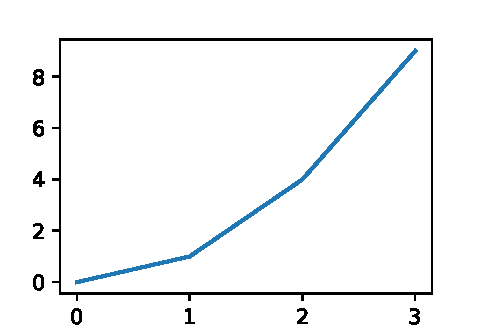
\includegraphics[width=0.6\linewidth]{figures/kinds.figure.pdf}\par
% alt: A rising curve
\setcounter{figure}{0}\captionof{figure}{y = x squared}
\vspace{12pt}
\end{samepage}
\end{adjustwidth}

\end{document}
